\iffalse
\let\negmedspace\undefined
\let\negthickspace\undefined
\documentclass[journal,12pt,twocolumn]{IEEEtran}

\usepackage{cite}
\usepackage{amsmath,amssymb,amsfonts,amsthm}
\usepackage{graphicx}
\usepackage{textcomp}
\usepackage{xcolor}
\usepackage{txfonts}
\usepackage{listings}
\usepackage{enumitem}
\usepackage{mathtools}
\usepackage{gensymb}
\usepackage[breaklinks=true]{hyperref}
\usepackage{tkz-euclide} % loads  TikZ and tkz-base
\usepackage{listings}
\usepackage{circuitikz}
\usepackage{graphicx}

%\newcounter{MYtempeqncnt}
\DeclareMathOperator*{\Res}{Res}
%\renewcommand{\baselinestretch}{2}
\renewcommand\thesection{\arabic{section}}
\renewcommand\thesubsection{\thesection.\arabic{subsection}}
\renewcommand\thesubsubsection{\thesubsection.\arabic{subsubsection}}

\renewcommand\thesectiondis{\arabic{section}}
\renewcommand\thesubsectiondis{\thesectiondis.\arabic{subsection}}
\renewcommand\thesubsubsectiondis{\thesubsectiondis.\arabic{subsubsection}}

% correct bad hyphenation here
\hyphenation{op-tical net-works semi-conduc-tor}
\def\inputGnumericTable{}                                 %%

\lstset{
	frame=single,
	breaklines=true,
	columns=fullflexible
}



\newtheorem{theorem}{Theorem}[section]
\newtheorem{problem}{Problem}
\newtheorem{proposition}{Proposition}[section]
\newtheorem{lemma}{Lemma}[section]
\newtheorem{corollary}[theorem]{Corollary}
\newtheorem{example}{Example}[section]
\newtheorem{definition}[problem]{Definition}
\newcommand{\BEQA}{\begin{eqnarray}}
	\newcommand{\EEQA}{\end{eqnarray}}
\newcommand{\define}{\stackrel{\triangle}{=}}
\newcommand\figref{Fig.~\ref}
\newcommand\tabref{Table~\ref}
\bibliographystyle{IEEEtran}
%\bibliographystyle{ieeetr}


\providecommand{\mbf}{\mathbf}
\providecommand{\pr}[1]{\ensuremath{\Pr\left(#1\right)}}
\providecommand{\qfunc}[1]{\ensuremath{Q\left(#1\right)}}
\providecommand{\sbrak}[1]{\ensuremath{{}\left[#1\right]}}
\providecommand{\lsbrak}[1]{\ensuremath{{}\left[#1\right.}}
\providecommand{\rsbrak}[1]{\ensuremath{{}\left.#1\right]}}
\providecommand{\brak}[1]{\ensuremath{\left(#1\right)}}
\providecommand{\lbrak}[1]{\ensuremath{\left(#1\right.}}
\providecommand{\rbrak}[1]{\ensuremath{\left.#1\right)}}
\providecommand{\cbrak}[1]{\ensuremath{\left\{#1\right\}}}
\providecommand{\lcbrak}[1]{\ensuremath{\left\{#1\right.}}
\providecommand{\rcbrak}[1]{\ensuremath{\left.#1\right\}}}
\theoremstyle{remark}
\newtheorem{rem}{Remark}
\newcommand{\sgn}{\mathop{\mathrm{sgn}}}
\providecommand{\abs}[1]{\left\vert#1\right\vert}
\providecommand{\res}[1]{\Res\displaylimits_{#1}}
\providecommand{\norm}[1]{\left\lVert#1\right\rVert}
%\providecommand{\norm}[1]{\lVert#1\rVert}
\providecommand{\mtx}[1]{\mathbf{#1}}
\providecommand{\mean}[1]{E\left[ #1 \right]}
\providecommand{\fourier}{\overset{\mathcal{F}}{ \rightleftharpoons}}
%\providecommand{\hilbert}{\overset{\mathcal{H}}{ \rightleftharpoons}}
\providecommand{\system}{\overset{\mathcal{H}}{ \longleftrightarrow}}
%\newcommand{\solution}[2]{\textbf{Solution:}{#1}}
\newcommand{\solution}{\noindent \textbf{Solution: }}
\newcommand{\cosec}{\,\text{cosec}\,}
\providecommand{\dec}[2]{\ensuremath{\overset{#1}{\underset{#2}{\gtrless}}}}
\newcommand{\myvec}[1]{\ensuremath{\begin{pmatrix}#1\end{pmatrix}}}
\newcommand{\mydet}[1]{\ensuremath{\begin{vmatrix}#1\end{vmatrix}}}
\renewcommand{\abstractname}{Question}

\let\vec\mathbf

	
	\vspace{3cm}
	
	


\newcommand{\permcomb}[4][0mu]{{{}^{#3}\mkern#1#2_{#4}}}
\newcommand{\comb}[1][-1mu]{\permcomb[#1]{C}}

%\IEEEpeerreviewmaketitle

\newcommand \tab [1][1cm]{\hspace*{#1}}
%\newcommand{\Var}{$\sigma ^2$}
\usepackage{amssymb}
\usepackage{amsmath}
\title{
	
\title{NCERT Mathematics 11.9.3 Q32}
\author{EE23BTECH11213 - MUTHYALA NIKHITHA SRI
}


}
\begin{document}

\maketitle

\textbf{Question:} 
If A.M. and G.M. of roots of a quadratic equation are 8 and 5,respectively,then obtain the quadratic equation.

\textbf{Solution: }
\fi

\begin{table}[h]
 	\centering
 	\resizebox{6 cm}{!}{
 		  \begin{tabular}{|c|c|c|}
        \hline
        \textbf{Parameter} & \textbf{Description} & \textbf{Value} \\
        \hline
        $ x_1, x_2 $ & Roots of a quadratic equation & ?  \\
        \hline
        $\frac{x_1 + x_2}{2}$& A.M. of roots & 8 \\
        \hline
        $\sqrt{x_1 \cdot x_2}$& G.M. of roots & 5 \\
        \hline
    \end{tabular}


 	}
 	\caption{Input Parameters}
    \label{tab:table_9.3.32}
 \end{table}


\begin{align}
x_1 \cdot x_2 &= 25 \\
x_1 + x_2 &= 16 \\
\implies  x^2 - 16x + 25 &= 0 \\
\implies x_1 &= 8+\sqrt{39} \\
\implies x_2 &= 8-\sqrt{39} 
\end{align}

For AP, 
\begin{align}
x\brak{0} &= 8+\sqrt{39} \\
d &= -2\sqrt{39} \\
x\brak{n} &= \brak{8+\sqrt{39} + n\brak{-2\sqrt{39}}}u\brak{n} \\
X\brak{z} &= \frac{8+\sqrt{39}}{1 - z^{-1}} + \frac{\brak{-2\sqrt{39}}\cdot z^{-1}}{\brak{1 - z^{-1}}^2}  \quad \abs{z} > \abs{1} \\
\implies X\brak{z} &= \frac{8+\sqrt{39}-\brak{8+3\sqrt{39}}\cdot{z^{-1}}}{\brak{1 - z^{-1}}^2} \quad \abs{z} > \abs{1}
\end{align}

For GP,
\begin{align}
x\brak{0} &= 8+\sqrt{39} \\
r &= \frac{8-\sqrt{39}}{8+\sqrt{39}} \\
x\brak{n} &= \brak{\brak{8+\sqrt{39}}\cdot {\brak{\frac{8-\sqrt{39}}{8+\sqrt{39}}}}^{n}}u\brak{n} \\
X\brak{z} &= \frac{8+\sqrt{39}}{1-\frac{\brak{8-\sqrt{39}}z^{-1}}{8+\sqrt{39}}} \quad \abs{z} > \frac{103-16\sqrt{39}}{25}
\end{align}

\begin{figure}[h!]
    \centering
    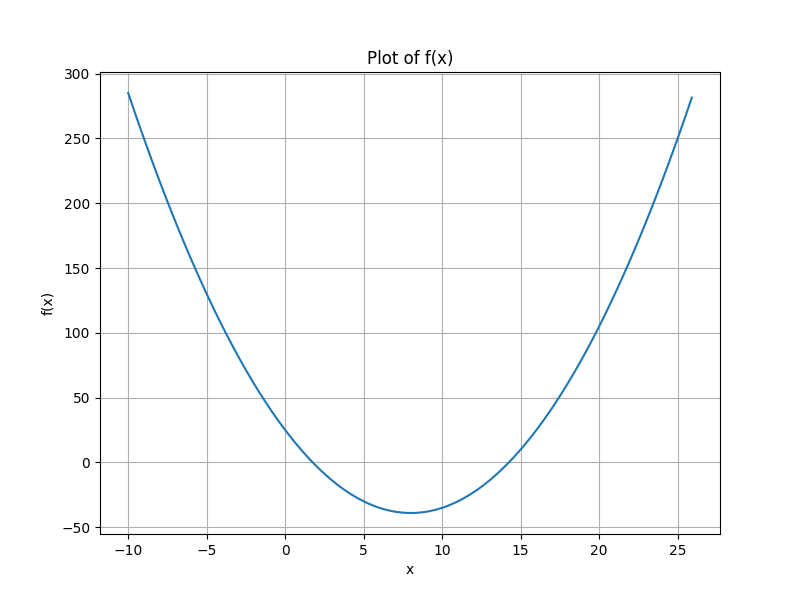
\includegraphics[width=\columnwidth]{ncert-maths/11/9/3/32/figs/f1.png}
    \caption{Plot of $f\brak{x} = x^2 - 16x + 25 = 0$}
    \label{fig: nik1}
\end{figure}

\begin{figure}[h!]
    \centering
    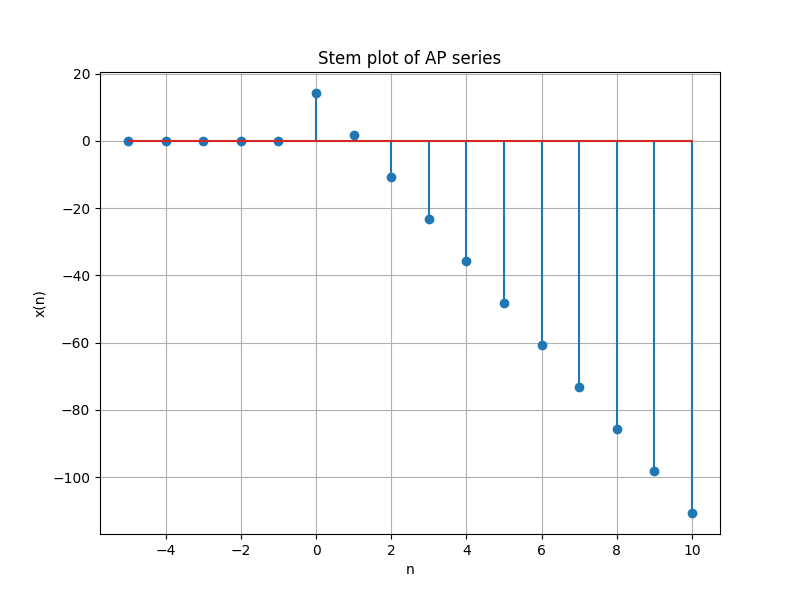
\includegraphics[width=\columnwidth]{ncert-maths/11/9/3/32/figs/ap.png}
    \caption{Plot of $x\brak{n} = \brak{8+\sqrt{39} + n\brak{-2\sqrt{39}}}u\brak{n}$}
    \label{fig: nik2}
\end{figure}

\begin{figure}[h!]
    \centering
    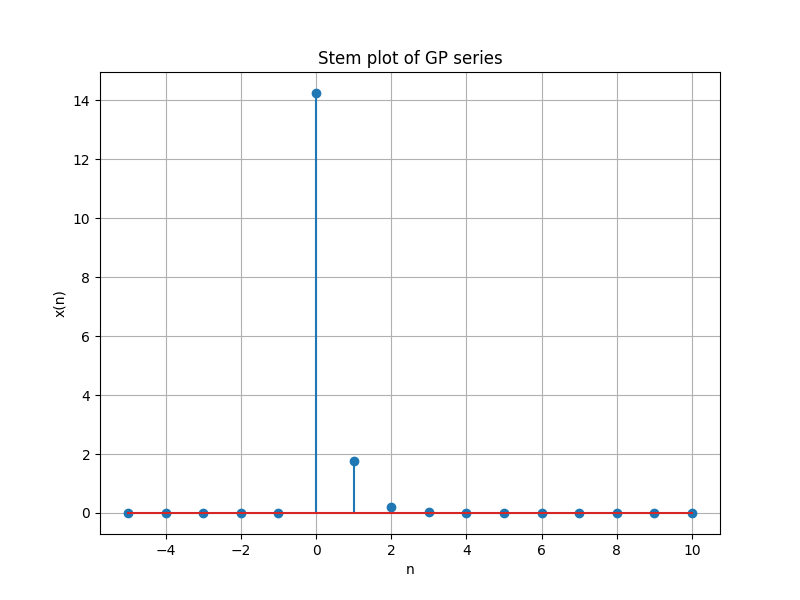
\includegraphics[width=\columnwidth]{ncert-maths/11/9/3/32/figs/gp.png}
    \caption{Plot of $x\brak{n} = \brak{\brak{8+\sqrt{39}}\cdot {\brak{\frac{8-\sqrt{39}}{8+\sqrt{39}}}}^{n}}u\brak{n}$}
    \label{fig: nik3}
\end{figure}

%\end{document}
